\documentclass[a4paper]{article}

\usepackage[utf8x]{inputenc}    
\usepackage[T1]{fontenc}
\usepackage[spanish]{babel}
\usepackage{multicol}

\usepackage{wrapfig}
\usepackage{graphicx}

\usepackage{bm}
\usepackage{amsxtra} 
\usepackage{amssymb}% to get the \mathbb alphabet
\usepackage{amsmath}

\usepackage[box,completemulti,separateanswersheet]{automultiplechoice}    
\def\AMCformQuestion#1{\vspace{\AMCformVSpace}\par {\sc Pregunta #1:} }    
\def\AMCbeginQuestion#1#2{\par\noindent{\bf Pregunta #1}#2\hspace*{1em}}
\def\AMCcleardoublepage{\ifodd\thepage\clearpage\mbox{}\fi\clearpage}

\begin{document}

\AMCrandomseed{1237893}

%%%%%%%%%%%%%%%%%%%%%%%%%%%%%%%%%%%%%%%%%%%%%%%%%%%%%%%%%%%%%%%%%%%%%%%%%%%%%
\element{test1}{
\begin{question}{P1}
Indicar aproximadamente el desplazamiento vertical del nodo situado en la esquina superior izquierda:
\begin{multicols}{2} 
\begin{choices}
     \correctchoice{$0.2$ mm}
     \wrongchoice{$0.2$ cm }
     \wrongchoice{$3.3$ mm }
     \wrongchoice{$3.3$ cm }
    \end{choices}
\end{multicols}
\end{question}
}
%%%%%%%%%%%%%%%%%%%%%%%%%%%%%%%%%%%%%%%%%%%%%%%%%%%%%%%%%%%%%%%%%%%%%%%%%%%%%
\element{test1}{
\begin{question}{P2}
Indicar aproximadamente el desplazamiento horizontal del nodo situado en la esquina superior derecha:
\begin{multicols}{2} 
\begin{choices}
     \correctchoice{$2.8$ mm}
     \wrongchoice{$2.8$ cm }
     \wrongchoice{$1.6$ mm }
     \wrongchoice{$1.6$ cm }
    \end{choices}
\end{multicols}
\end{question}
}
%%%%%%%%%%%%%%%%%%%%%%%%%%%%%%%%%%%%%%%%%%%%%%%%%%%%%%%%%%%%%%%%%%%%%%%%%%%%%
\element{test1}{
\begin{question}{P3}
Indicar aproximadamente el m\'aximo valor obtenido de la tensi\'on $\sigma_{yy}$:
\begin{multicols}{2} 
\begin{choices}
     \correctchoice{$42.2$ MPa}
     \wrongchoice{$12.61$ MPa}
     \wrongchoice{$0.561$ MPa}
     \wrongchoice{$27.13$ MPa}
    \end{choices}
\end{multicols}
\end{question}
}
%%%%%%%%%%%%%%%%%%%%%%%%%%%%%%%%%%%%%%%%%%%%%%%%%%%%%%%%%%%%%%%%%%%%%%%%%%%%%
\element{test1}{
\begin{question}{P4}
Indicar la localización en la que se obtiene el valor m\'inimo (compresi\'on) de
$\sigma_{xx}$:
\begin{choices}
     \correctchoice{A lo largo del arco inferior}
     \wrongchoice{A lo largo del arco superior}
     \wrongchoice{Esquina superior izquierda}
     \wrongchoice{Esquina superior derecha}
    \end{choices}
\end{question}
}
%%%%%%%%%%%%%%%%%%%%%%%%%%%%%%%%%%%%%%%%%%%%%%%%%%%%%%%%%%%%%%%%%%%%%%%%%%%%%
\element{test1}{
\begin{question}{P5}
Indicar aproximadamente el valor de la reacci\'on horizontal en el lado derecho del apoyo derecho:
\begin{multicols}{2} 
\begin{choices}
     \correctchoice{$-2.42$ MN}
     \wrongchoice{$-7.53$ MN}
     \wrongchoice{$-17.71$ MN}
     \wrongchoice{$-30.43$ MN}
    \end{choices}
\end{multicols}
\end{question}
}
%%%%%%%%%%%%%%%%%%%%%%%%%%%%%%%%%%%%%%%%%%%%%%%%%%%%%%%%%%%%%%%%%%%%%%%%%%%%%
\element{test1}{
\begin{question}{P6}
Indicar aproximadamente el valor de la reacci\'on vertical en el lado izquierdo del apoyo izquierdo:
\begin{multicols}{2} 
\begin{choices}
     \correctchoice{$0.85$ MN}
     \wrongchoice{$10.6$ MN}
     \wrongchoice{$-31.2$ MN}
     \wrongchoice{$-3.25$ MN}
    \end{choices}
\end{multicols}
\end{question}
}
%%%%%%%%%%%%%%%%%%%%%%%%%%%%%%%%%%%%%%%%%%%%%%%%%%%%%%%%%%%%%%%%%%%%%%%%%%%%%%
\element{test1}{
\begin{question}{P7}
Las tensiones horizontales se encuentran entre:
\begin{multicols}{2}
\begin{choices}
	\correctchoice{$-40.00$ y $40.00$ MPa}
	\wrongchoice{$-50.00$ y $10.00$ MPa}
	\wrongchoice{$-20.00$ y $25.00$ MPa}
	\wrongchoice{$5.0$ y $190.00$ MPa}
\end{choices}
\end{multicols}
\end{question}
}
%%%%%%%%%%%%%%%%%%%%%%%%%%%%%%%%%%%%%%%%%%%%%%%%%%%%%%%%%%%%%%%%%%%%%%%%%%%%%%
\element{test1}{
\begin{question}{p8}
En general, en un problema plano de elasticidad lineal con la hipótesis de deformación plana:
\begin{multicols}{2}
\begin{choices}
       \correctchoice{Los desplazamientos perpendiculares al plano del sólido son
nulos}
        \wrongchoice{Las tensiones perpendiculares al plano del sólido son
nulas}
        \wrongchoice{Las tensiones y las deformaciones perpendiculares al plano
del sólido son nulas}
        \wrongchoice{Las deformaciones en dirección perpendicular al plano son
        nulas pero los movimientos en dicha dirección son no nulos}
\end{choices}
\end{multicols}
\end{question}
}
%%%%%%%%%%%%%%%%%%%%%%%%%%%%%%%%%%%%%%%%%%%%%%%%%%%%%%%%%%%%%%%%%%%%%%%%%%%%%%
\element{test1}{
\begin{question}{p9}
En un problema plano se quiere integrar de manera exacta el polinomio:
$$p(x,y)=x^3+y^3+xy$$
La cuadratura de Gauss que debe utizarse debe tener como mínimo:
\begin{choices}
        \correctchoice{$2 \times 2$ puntos de Gauss}
        \wrongchoice{$1 \times 1$ punto de Gauss}
        \wrongchoice{$3 \times 3$ puntos de Gauss}
        \wrongchoice{Con una cuadratura de Gauss no se puede hacer la integral exacta;
        siempre proporcionará un resultado aproximado al exacto}
\end{choices}
\end{question}
}
%%%%%%%%%%%%%%%%%%%%%%%%%%%%%%%%%%%%%%%%%%%%%%%%%%%%%%%%%%%%%%%%%%%%%%%%%%%%%%
\element{test1}{
\begin{question}{p10}
En un problema de flujo en medios porosos, la variable primaria que se obtiene
al resolver la ecuación de elementos finitos $\bm{K} \bm{d}=\bm{f}$ es:
\begin{multicols}{2}
\begin{choices}
        \correctchoice{la altura piezométrica $z+p/\gamma$, siendo $z$ la altura geométrica y $p/\gamma$
        la altura de presión ($p$ presión y $\gamma$ peso específico)}
        \wrongchoice{La presión}
        \wrongchoice{La temperatura}
        \wrongchoice{La velocidad del fluido}
\end{choices}
\end{multicols}
\end{question}
}
%%%%%%%%%%%%%%%%%%%%%%%%%%%%%%%%%%%%%%%%%%%%%%

\scoringDefaultS{b=1,m=-1/(N-1)}

\onecopy{10}{    

%%% beginning of the test sheet header:    

\noindent{\large\bf Método de los Elementos Finitos  \hfill MUECYM \hfill FINAL ORD. \# Ej 1}
\begin{center}
%\vspace*{.1cm}
%Se atribuirá puntuación negativa a las respuestas incorrectas.\\
\vspace*{.1cm}
20 ene 2025. \hspace{7cm} Tiempo: 45 minutos.\\


\end{center}

\vspace{1ex}

La estructura de la figura está sometida a las dos cargas que se representan en la misma, una carga de viento repartida $q$ y una carga puntual $P$, con las condiciones de sustentación y dimensiones que también se indican en dicha figura. En el apoyo derecho se restringen los movimientos horizontales y verticales, mientras que en el izquierdo solo se restringen los verticales.

\begin{center}
  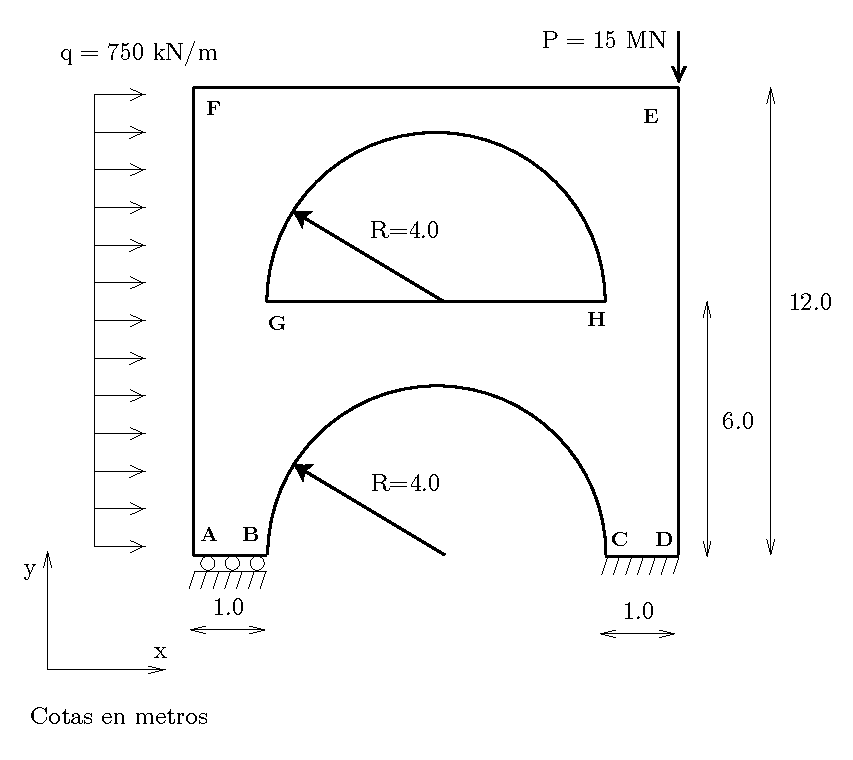
\includegraphics[width=0.7\linewidth]{figura}
\end{center}

Las propiedades mecánicas son $E=220$ GPa y $\nu=0.19$. El espesor
es igual a $1.0$ m y se supone la hipótesis de tensión plana. Para generar la malla se empleará un tamaño de malla igual a $0.6$ m. La malla estará compuesta únicamente por cuadriláteros (\textit{Quad}), con interpolación cuadrática e integración reducida, resultando elementos tipo \textit{CPS8R}.

\vspace{4mm}
\hrulefill
\vspace{4mm}

%%% end of the header

\shufflegroup{test1}
\insertgroup{test1}

%\AMCcleardoublepage    
\clearpage

\AMCformBegin    

%%% beginning of the answer sheet header

\noindent\AMCcode{nummat}{2}\hspace*{\fill}
\begin{minipage}{.7\linewidth}
$\longleftarrow{}$ Escriba su número de matrícula marcando los dígitos
en los recuadros (con ceros a la izquierda si el número es de menos de dos dígitos) y el nombre y apellidos debajo.

\vspace{3ex}

\namefield{\fbox{
   \begin{minipage}{.9\linewidth}
     Apellidos, Nombre:

     \vspace*{.5cm}\dotfill
     \vspace*{1mm}
   \end{minipage}
 }}
\end{minipage}

\begin{center}
 \bf\em Debe dar las respuestas exclusivamente en esta hoja (las respuestas en las demás hojas no serán tenidas en cuenta).
\end{center}

%%% end of the answer sheet header


\AMCform    

\AMCcleardoublepage    

}  

\end{document}
